\documentclass[12pt,a4paper]{article}

% --- PACKAGES ---
\usepackage[margin=2.5cm]{geometry}
\usepackage{amsmath, amssymb, amsfonts}
\usepackage{graphicx}
\usepackage{booktabs}
\usepackage{xcolor}
\usepackage{listings}
\usepackage{enumitem}
\usepackage{fancyhdr}
\usepackage{hyperref}
\usepackage{tikz}
\usepackage{circuitikz}
\usetikzlibrary{calc, shadows}
\usepackage{float}
\usepackage{array}
\usepackage{multirow}

% --- THEME COLORS ---
\definecolor{SharifRed}{RGB}{185, 4, 0}
\definecolor{SharifDark}{RGB}{40, 45, 55}
\definecolor{SharifLight}{RGB}{174, 174, 174}
\definecolor{CalcGray}{RGB}{245, 245, 245}
\definecolor{CodeGreen}{RGB}{0, 150, 0}
\definecolor{CodeBlue}{RGB}{0, 0, 200}

% --- TCOLORBOX CONFIGURATION ---
\usepackage{tcolorbox}
\tcbuselibrary{skins, breakable}

% 1. Task Box
\newtcolorbox{taskbox}[2][]{
    colback=SharifRed!5!white,
    colframe=SharifRed,
    coltitle=white,
    fonttitle=\bfseries\large,
    title={#2},
    arc=0mm,
    boxrule=1.5pt,
    enhanced jigsaw,
    breakable,
    drop shadow={opacity=0.25,shadow xshift=2pt,shadow yshift=-2pt},
    #1
}

% 2. Answer Box
\newtcolorbox{answerbox}[2][]{
    colback=white,
    colframe=SharifDark,
    coltitle=white,
    fonttitle=\bfseries\large,
    title={#2},
    arc=0mm,
    boxrule=1pt,
    enhanced jigsaw,
    breakable,
    lines before break=1,
    drop shadow={opacity=0.15,shadow xshift=1pt,shadow yshift=-1pt},
    #1
}

% 3. Calculation Box
\newtcolorbox{calcbox}[2][]{
    colback=CalcGray,
    colframe=SharifLight,
    coltitle=black,
    fonttitle=\bfseries\large,
    title={#2},
    arc=0mm,
    boxrule=1.5pt,
    borderline={0.5pt}{0pt}{black!30!white,dashed},
    enhanced jigsaw,
    breakable,
    lines before break=1,
    drop shadow={opacity=0.15,shadow xshift=1pt,shadow yshift=-1pt},
    #1
}

% --- LISTINGS CONFIGURATION ---
\lstset{
    language=Python,
    backgroundcolor=\color{CalcGray},
    basicstyle=\ttfamily\scriptsize\selectfont,
    keywordstyle=\color{CodeBlue}\bfseries,
    commentstyle=\color{CodeGreen}\itshape,
    stringstyle=\color{SharifRed},
    showstringspaces=false,
    breaklines=true,
    numbers=left,
    numberstyle=\tiny\color{gray},
    frame=single,
    rulecolor=\color{SharifLight}
}

% --- PERSIAN LANGUAGE SUPPORT ---
\usepackage{xepersian}
\settextfont{XB Niloofar.ttf}
\setdigitfont{XB Niloofar.ttf}

% --- HEADER/FOOTER ---
\setlength{\headheight}{15pt}
\pagestyle{fancy}
\fancyhf{}
\rhead{\textcolor{SharifRed}{\textbf{گزارش پروژه الکترونیک ۲: طراحی تقویت‌کننده}}}
\lhead{\textcolor{SharifRed}{\textbf{الکترونیک ۲}}}
\cfoot{\thepage}
\renewcommand{\headrulewidth}{1pt}
\renewcommand{\headrule}{\hbox to\headwidth{\color{SharifRed}\leaders\hrule height \headrulewidth\hfill}}

% --- HYPERLINKS SETUP ---
\hypersetup{
    colorlinks=true,
    linkcolor=SharifRed,
    urlcolor=cyan,
    pdftitle={Electronics 2 Project Report Template},
}

\begin{document}

% =============================================================================
% TITLE
% =============================================================================
\begin{center}
    \vspace*{0.5cm}
    {\huge \textbf{\textcolor{SharifDark}{گزارش طراحی و شبیه‌سازی پروژه الکترونیک ۲\\(فاز اول)}}} \\
    \vspace{0.5cm}
    \begin{tabular}{r l r l}
        \textbf{نام و نام خانوادگی:} & \underline{ آریا فاتح کرداری} & \textbf{شماره دانشجویی:} & \underline{403110382} \\
    \end{tabular}
    \vspace{1cm}
    \hrule
\end{center}

\vspace{0.5cm}

% =============================================================================
% PROJECT REQUIREMENTS
% =============================================================================
\section{مشخصات مورد نیاز پروژه}

\begin{taskbox}{الزامات طراحی}
در این پروژه باید یک تقویت‌کننده طراحی شود که مشخصات زیر را برآورده کند:
\begin{center}
\begin{tabular}{c l}
\toprule
\textbf{مقدار} & \textbf{پارامتر} \\
\midrule
$1mV$ & ولتاژ ورودی ($V_{in}$) \\
$500\Omega$ & مقاومت بار ($R_{Load}$) \\
$+10V,\,-10V$ & ولتاژهای تغذیه ($V_{CC},V_{EE}$) \\
$>54dB$ & بهره تفاضلی ($A_{vd}$) \\
$>80dB$ & نسبت پس‌زنی حالت مشترک ($CMRR$) \\
$6V$ & تغییرات دامنه‌ی خروجی پیک تا پیک \\
$>50k\Omega$ & مقاومت ورودی ($R_{in}$) \\
$<5k\Omega$ & مقاومت خروجی ($R_{out}$) \\
$<60mW$ & توان مصرفی حالت سکون (بدون بار) \\
\bottomrule
\end{tabular}
\end{center}
\end{taskbox}

\begin{answerbox}{جدول نهایی بررسی مشخصات}
در انتهای طراحی، نتایج نهایی خود را در جدول زیر وارد کنید.
\begin{center}
\begin{tabular}{|c|c|c|}
\hline
\textbf{پارامتر} & \textbf{مقدار موردنیاز} & \textbf{مقدار طراحی‌شده}  \\
\hline
$A_{vd}$ & $>54dB$ & $103 \, dB$ \\
\hline
$CMRR$ & $>80dB$ & $89 \, dB$\\
\hline
Swing & $6V_{pp}$ & $6.7$\\
\hline
$R_{in}$ & $>50k\Omega$ & $150 \, \text{k}\Omega$ \\
\hline
$R_{out}$ & $<5k\Omega$ & $3 \omega$\\
\hline
$P_Q$ & $<60mW$ & $47.4 \, \text{mW}$\\
\hline
Cost & $\le 200$ & $180$\\
\hline
\end{tabular}
\end{center}
\end{answerbox}

\newpage

% =============================================================================
% SECTION 1
% =============================================================================
\section{معرفی ساختار مدار و طراحی اولیه}

\begin{taskbox}{خواسته مسئله (بخش ۱)}
ساختار کلی تقویت‌کننده طراحی‌شده را معرفی کنید. مشخص کنید مدار شما شامل چه بخش‌هایی است:
\begin{itemize}
    \item طبقه ورودی
    \item طبقه یا طبقات میانی
    \item بافر یا خروجی مورد استفاده در فاز اول
    \item شبکه بایاس و آینه‌های جریان
\end{itemize}
همچنین توضیح دهید چرا این ساختار را انتخاب کرده‌اید.
\end{taskbox}

\begin{answerbox}{معرفی ساختار انتخابی}
	\begin{enumerate}
		\item \textbf{ساختار ورودی:}
		از یک زوج تفاضلی \lr{BJT} استفاده شده است با مقاومت‌های امیتر. خروجی‌ مدار ورودی به طبقه‌ی بعدی تقویت وصل شده است با بار فعال. تقویت عمده در این طبقه انجام می‌شود. طبقه‌‌های بعدی بافر هستند و تقویتی انجام نمی‌دهند.
		\item 
		\textbf{طبقه میانی:}
		از یک بافر BJT استفاده شده است. بافر باعث می‌شود که ضریب تقویت ولتاژ پس از اتصال به طبقه بعدی افت پیدا نکند. در این طبقه مقدار DC هم به میزان خوبی تنظیم می‌گردد که در نهایت سویینگ مناسبی بدهد. مقاومت $R_7$ مقدار DC خروجی را به میزانی مناسبی افزایش می‌دهد.
		\item 
		\textbf{بافر خروجی:}
			طبقه خروجی از یک مدار کالکتور مشترک استفاده شده است. استفاده از دو ترانزیستور برای این بخش، به شدت مقاومت خروجی را کاهش می‌دهد و باعث می‌شود که ضریب تقویت در خروجی افت پیدا نکند.  
	\end{enumerate}
	شبکه بایاس از آینه جریان و منبع جریان Widlar تشکیل شده است. تمامی ترانزیستور‌های شبکه بایاس BJT هستند. میزان جریان با استفاده از دو مقاومت $R_3$ و $R_8$ تعیین می‌گردد.
	می‌توان با تغییر این دو مقاومت، ضریب تقویت و خصوصیات مدار را تغییر داد و در عوض بهای آن را با مصرف بیشتر توان پرداخت.
	
	
	استفاده از BJT به ما بهره بیشتر در نتیجه نویز پایین‌تری نسبت به MOS می‌دهد. به این دلیل در تمام طراحی از BJT استفاده شده است. 
	به دلیل اینکه در طبقه تقویت اول از ترانزیستور‌های \lr{NPN} استفاده شده، سعی شده است که در طبقات بعدی از \lr{PNP} استفاده شود که مقدار DC مدار به نوعی کنترل شود.
\end{answerbox}

\begin{answerbox}{شماتیک کامل مدار}
\begin{center}
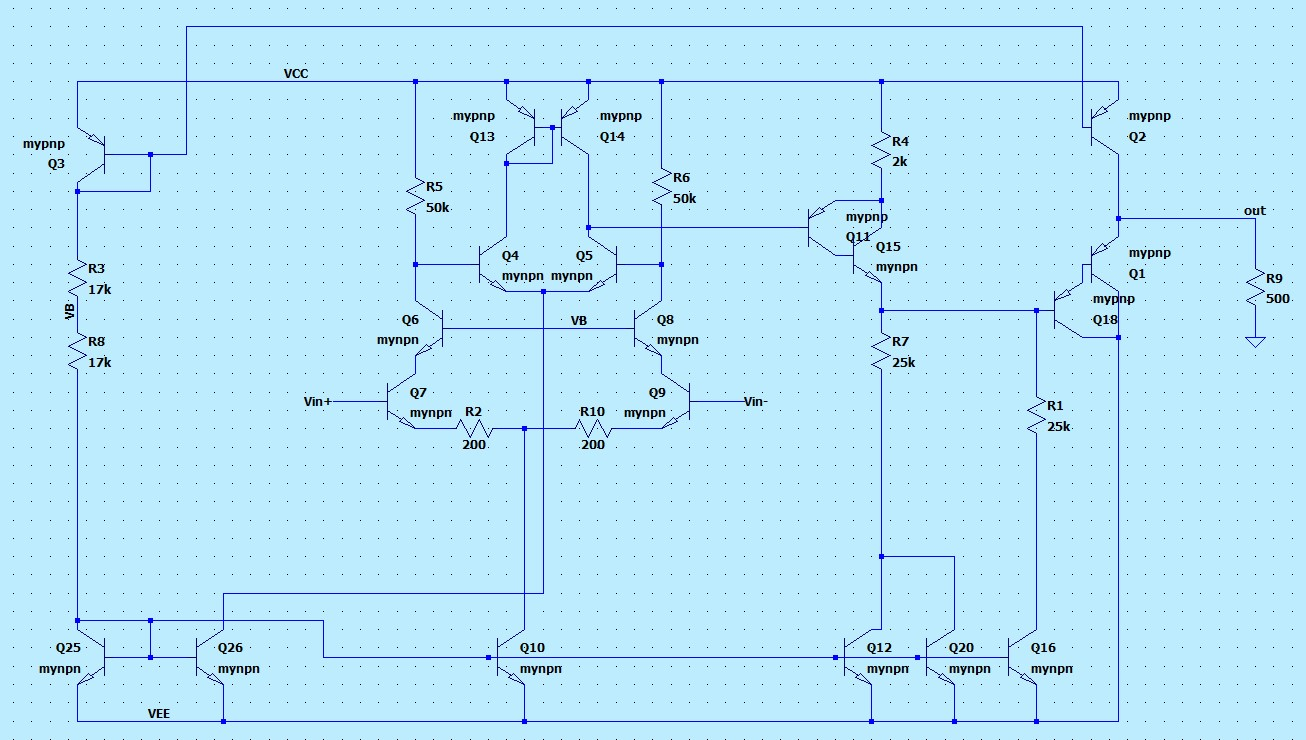
\includegraphics[width = \textwidth]{Scheme.jpg}
\end{center}
\end{answerbox}

\newpage

% =============================================================================
% SECTION 2
% =============================================================================
\section{تحلیل DC و طراحی بایاس}

\begin{taskbox}{خواسته مسئله (بخش ۲)}
برای مدار خود تحلیل DC انجام دهید. نقطه کار طبقات مختلف، ولتاژ گره‌ها و جریان شاخه‌های اصلی را بدست آورید و با تحلیل تئوری مقایسه کنید.
\end{taskbox}

\begin{calcbox}{محاسبات تئوری بایاس}
	در محاسبات، $V_{BE} = 0.65 \, V$ در نظر گرفته شده است.
برای محاسبه از سمت چپ مدار شروع می‌کنیم. 
$$I_{ref} = \frac{20 - 1.3}{17\times2 \, k \Omega} = 550 \, \mu A$$
در نتیجه برای ترانزیستور‌های ورودی تفاضلی داریم:
$$IC_{7} = IC_6 = 275 \, \mu A$$
برای طرف دیگر تفاضلی هم مقادیر به همین شکل است. 
$$IC_4 = IC_5 = 275 \, \mu A$$
به دلیل آینه جریان، جریان گذرنده از Q15:
$$IC_{15} = 550 \, \mu A$$
$$IC_{11} =\frac{IC_{15}}{200} =  2.8 \, \mu A$$
طبقه بافر خروجی:
$$IC_{1} = 550 \, \mu A$$
$$IC_{18} = 3.7 \, \mu A$$
\end{calcbox}

\begin{answerbox}{نتایج شبیه‌سازی DC Operating Point}
همانطور که در شکل زیر مشهود است، مقادیر محاسبه شده در تئوری و مقادیر شبیه سازی گاها تفاوت زیادی دارند. به این دلیل می‌تواند باشد که برای مثال اثر ارلی در محاسبات تئوری در نظر گرفته نشده است.
\begin{center}
 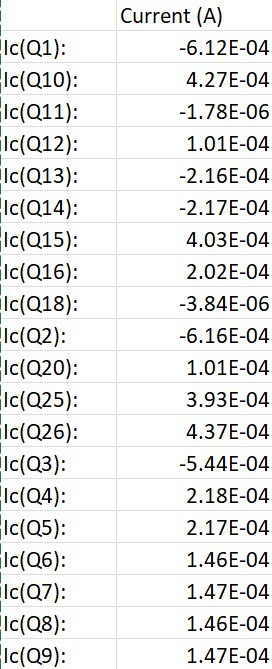
\includegraphics[width=0.5\textwidth]{Bias.jpg}
\end{center}
\end{answerbox}



\newpage

% =============================================================================
% SECTION 3
% =============================================================================
\section{تحلیل بهره تفاضلی}

\begin{taskbox}{خواسته مسئله (بخش ۳)}
بهره تفاضلی مدار را بدست آورید. برای این منظور ورودی تفاضلی مناسب اعمال کرده و مقدار $A_{vd}$ را محاسبه کنید. نتیجه باید با شرط $A_{vd}>54dB$ مقایسه شود.
\end{taskbox}

\begin{calcbox}{محاسبات تئوری بهره تفاضلی}
\subsection*{تحلیل طبقه اول (زوج تفاضلی با کاسکود)}
طبقه اول شامل زوج تفاضلی $Q_7$ و $Q_9$ با مقاومت‌های دژنراسیون $R_1 = R_{11} = 200 \Omega$ است. ابتدا هدایت انتقالی ($g_m$) ترانزیستورهای ورودی را محاسبه می‌کنیم:
\begin{align*}
	I_{C7} &= 150 \mu\text{A} \\
	g_{m1} &= \frac{I_{C7}}{V_T} = 5.81 \text{ mA/V}
\end{align*}
هدایت انتقالی موثر کل طبقه ($G_{m1}$) با در نظر گرفتن اثر دژنراسیون امیتر:
\begin{align*}
	G_{m1} = \frac{g_{m1}}{1 + g_{m1}R_1} = 2.69 \text{ mA/V}
\end{align*}
مقاومت بار دیده شده در خروجی این طبقه (کلکتور $Q_6$ و $Q_8$) برابر است با موازی شدن مقاومت $R_5$ و مقاومت ورودی طبقه بعد ($r_{\pi 4}$). از مقاومت خروجی بسیار بزرگ طبقه کاسکود صرف‌نظر شده است:
\begin{align*}
	I_{C4} &= 218 \mu\text{A} \implies g_{m4} = 8.45 \text{ mA/V} \\
	r_{\pi 4} &= \frac{\beta_n}{g_{m4}} = 23.67 \text{ k}\Omega \\
	R_{L1} &= R_5 \parallel r_{\pi 4} =  16.06 \text{ k}\Omega
\end{align*}
بنابراین بهره ولتاژ طبقه اول (از ورودی تفاضلی تا خروجی تفاضلی) برابر است با:
\begin{align*}
	A_{v1} &= G_{m1} \times R_{L1} =  43.21
\end{align*}

\subsection*{تحلیل طبقه دوم (زوج تفاضلی با بار فعال)}
این طبقه سیگنال تفاضلی را از طبقه اول گرفته و به صورت تک‌انتهایی (Single-Ended) در کلکتور $Q_5$ تحویل می‌دهد. هدایت انتقالی این طبقه برابر با $g_{m4}$ است که پیش‌تر محاسبه شد ($8.45 \text{ mA/V}$). 

مقاومت خروجی در این گره ($R_{out2}$) از موازی شدن مقاومت خروجی ترانزیستورهای $Q_5$ و $Q_{14}$ و مقاومت ورودی طبقه بعد ($R_{in3}$ متعلق به $Q_{11}$) به دست می‌آید. با استفاده از ولتاژ ارلی $V_A = 100 \text{ V}$:
\begin{align*}
	r_{o5} &= \frac{V_A}{I_{C5}} = \frac{100}{217\mu} \approx 461 \text{ k}\Omega \\
	r_{o14} &= \frac{V_A}{I_{C14}} = \frac{100}{217\mu} \approx 461 \text{ k}\Omega
\end{align*}
برای محاسبه مقاومت ورودی $Q_{11}$:
\begin{align*}
	I_{C11} &= 1.78 \mu\text{A} \implies g_{m11} = 0.069 \text{ mA/V} \\
	R_{in3} &\approx r_{\pi 11} = \frac{\beta_p}{g_{m11}} = 2.17 \text{ M}\Omega
\end{align*}
مقاومت معادل خروجی طبقه دوم:
\begin{align*}
	R_{out2} &= r_{o5} \parallel r_{o14} \parallel R_{in3} = 230 \text{ k}\Omega
\end{align*}
بهره ولتاژ طبقه دوم برابر است با:
\begin{align*}
	A_{v2} &= g_{m4} \times R_{out2} = 1950
\end{align*}


با فرض اینکه طبقات بعدی بهره تقریبا یک دارند(بافر هستند)، بهره ی دیفرانسیلی مدار برابر است با:
\begin{align*}
	A_d &= A_{v1} \times A_{v2}  \approx 84300 \\
	A_{d(\text{dB})} &\approx 98.5 \text{ dB}
\end{align*}

\end{calcbox}

\begin{answerbox}{شبیه‌سازی بهره تفاضلی}
دو منبع ولتاژ سینوسی با فرکانس یکسان و دامنه یکسان (ولی معکوس) درست می‌کنیم. به ورودی تفاضلی وصل می‌کنیم. 

\begin{center}

\includegraphics[width=\textwidth]{1.jpg}
\end{center}
\vspace{4cm}

\textbf{نتیجه نهایی:}
در فرکانس $1 kHz$ داریم:
\begin{itemize}
    \item بهره تفاضلی خطی: \underline{$140\times 10^3$ }
    \item بهره تفاضلی بر حسب دسی‌بل: \underline{$103 \, dB$}
\end{itemize} 
\end{answerbox}

\newpage

% =============================================================================
% SECTION 4
% =============================================================================
\section{تحلیل بهره حالت مشترک و CMRR}

\begin{taskbox}{خواسته مسئله (بخش ۴)}
بهره حالت مشترک مدار را بدست آورید و سپس نسبت پس‌زنی حالت مشترک را از رابطه
$$CMRR = \frac{A_{vd}}{A_{vc}}$$
محاسبه کنید. نتیجه باید با شرط $CMRR>80dB$ مقایسه شود.
\end{taskbox}

\begin{calcbox}{محاسبات تئوری CMRR}


\subsection*{تحلیل بهره مشترک طبقه اول ($A_{c1}$)}
طبقه اول شامل زوج تفاضلی $Q_7$ و $Q_9$ است که با منبع جریان $Q_{10}$ تغذیه می‌شوند. ابتدا مقاومت خروجی منبع جریان دم ($r_{o10}$) را محاسبه می‌کنیم. جریان این ترانزیستور برابر با مجموع جریان دو شاخه است:
\begin{align*}
	I_{C10} & = 430 \mu\text{A} \\
	R_{tail1} &= r_{o10} = \frac{V_A}{I_{C10}} = 230 \text{ k}\Omega
\end{align*}

هنگامی که سیگنال مشترک $v_{ic}$ اعمال می‌شود، ترانزیستورهای $Q_7$ و $Q_9$ با هم موازی شده و به عنوان یک طبقه امیتر مشترک با مقاومت دژنراسیون $2R_{tail1} + R_1$ عمل می‌کنند. سیگنال خروجی این طبقه در کلکتور $Q_6$ (یا $Q_8$) ظاهر می‌شود که مستقیماً به مقاومت $R_5$ متصل است. بهره مشترک تا خروجی این طبقه (ولتاژ گره بیس $Q_4$ و $Q_5$) برابر است با:
\begin{align*}
	A_{c1} &= \frac{v_{c6}}{v_{ic}} \approx \frac{-R_5}{2 R_{tail1} + R_1}
\end{align*}
از آنجا که $R_1 = 200 \Omega$ در مقایسه با $2r_{o10}$ بسیار ناچیز است، می‌توان از آن صرف‌نظر کرد:
\begin{align*}
	A_{c1} = -0.1
\end{align*}

\subsection*{تحلیل بهره مشترک طبقه دوم ($A_{c2}$)}
سیگنال حالت مشترک تقویت‌شده در طبقه اول، اکنون به عنوان ورودی مشترک به بیس‌های $Q_4$ و $Q_5$ اعمال می‌شود. این طبقه یک زوج تفاضلی با بار فعال آینه جریان ($Q_{13}, Q_{14}$) است. 

ابتدا مقاومت خروجی منبع جریان دم این طبقه ($Q_{26}$) را محاسبه می‌کنیم:
\begin{align*}
	I_{C26} &= 440 \mu\text{A} \\
	R_{tail2} &= r_{o26} = \frac{V_A}{I_{C26}} =  230 \text{ k}\Omega
\end{align*}

هدایت انتقالی ترانزیستور بار فعال ($Q_{13}$) برابر است با:
\begin{align*}
	g_{m13} &= \frac{I_{C13}}{V_T} = 8.37 \text{ mA/V}
\end{align*}

رابطه تقریبی بهره مشترک در این ساختار برابر است با:
\begin{align*}
	A_{c2} &\approx -\frac{1}{2 g_{m13} R_{tail2}} = 2.6 \times 10^{-4}
\end{align*}
$$A = 2.6 \times 10^{-5}$$
\end{calcbox}

\begin{answerbox}{نتایج شبیه‌سازی حالت مشترک}
مشابه قسمت قبل ولی این بار هر دو را یک سینوسی می‌دهیم و ولتاژ خروجی را اندازه‌گیری می‌کنیم.

\begin{center}


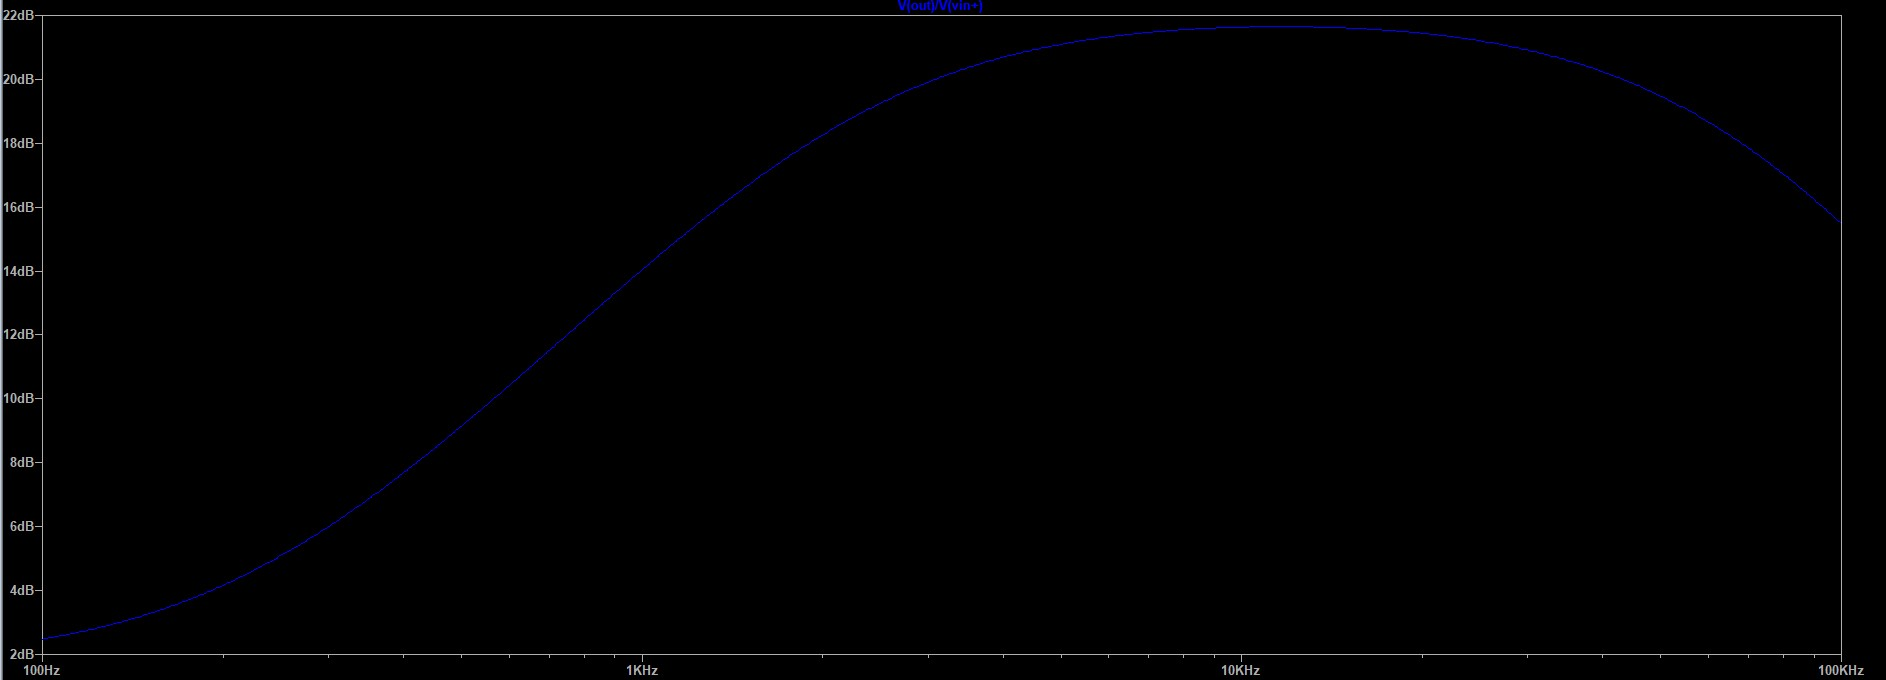
\includegraphics[width=0.85\textwidth]{CommonAC.jpg}
\end{center}
نتایج در فرکانس $1 kHz$.

\textbf{نتایج نهایی:}
\begin{itemize}
    \item بهره حالت مشترک $A_{vc}$: \underline{$5$}
    \item $CMRR$ خطی: \underline{$3.57\times 10^{-5}$}
    \item $CMRR$ بر حسب دسی‌بل: \underline{$-89\, dB$}
\end{itemize}
\end{answerbox}

\newpage

% =============================================================================
% SECTION 5
% =============================================================================
\section{تحلیل مقاومت ورودی}

\begin{taskbox}{خواسته مسئله (بخش ۵)}
مقاومت ورودی مدار را بدست آورید و با شرط $R_{in}>50k\Omega$ مقایسه کنید. روش اندازه‌گیری در شبیه‌سازی را به‌طور کامل توضیح دهید.
\end{taskbox}

\begin{calcbox}{محاسبات تئوری مقاومت ورودی}

مقاومت ورودی مدار، مقاومتی است که از دید منبع سیگنال تفاضلی در بیس‌های ترانزیستورهای $Q_7$ و $Q_9$ دیده می‌شود. به دلیل تقارن مدار، مقاومت ورودی کل برابر است با مجموع مقاومت دیده شده از هر بیس.


\begin{align*}
	I_{C7} &= 150 \mu\text{A} \\
	g_{m1} & =  5.81 \text{ mA/V} \\
	r_{\pi 7} &=  34.4 \text{ k}\Omega
\end{align*}

با توجه به وجود مقاومت‌های دژنراسیون امیتر ($R_1 = R_{11} = 200 \Omega$)، مقاومت دیده شده از بیس هر ترانزیستور:
\begin{align*}
	R_{in7} &= r_{\pi 7} + (\beta_n + 1) R_1 = 74.4 \text{ k}\Omega
\end{align*}
در نتیجه مقدار مقاومت ورودی دو برابر این مقدار است:
$$R_{in,diff} = 148.8 \text{ k}\Omega$$
\end{calcbox}

\begin{answerbox}{نتایج شبیه‌سازی مقاومت ورودی}
باید این اندازه‌گیری در حالت بی‌باری انجام شود. پس بار را حذف کرده و سپس مقاومت $R_S$ را در ورودی قرار می‌دهیم. می‌توانیم مقدار $R_S$ را با استفاده از \texttt{.step} تغییر داد به طوری که در ولتاژ ورودی نصف ولتاژ سیگنال ما بشود. آنگاه مقاومت ورودی و مقاومت $R_S$ برابر هستند.
\begin{center}
	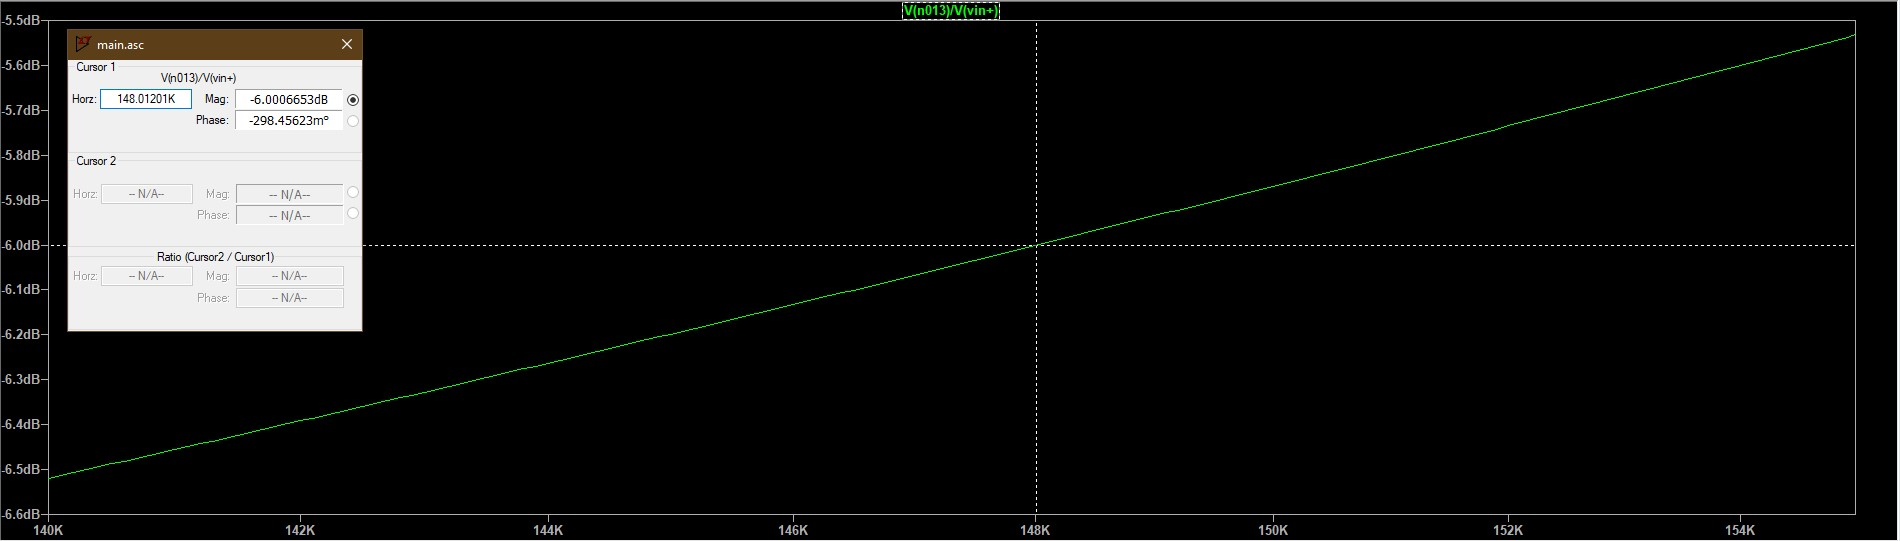
\includegraphics[width = \textwidth]{Rin_simulation.jpg}
	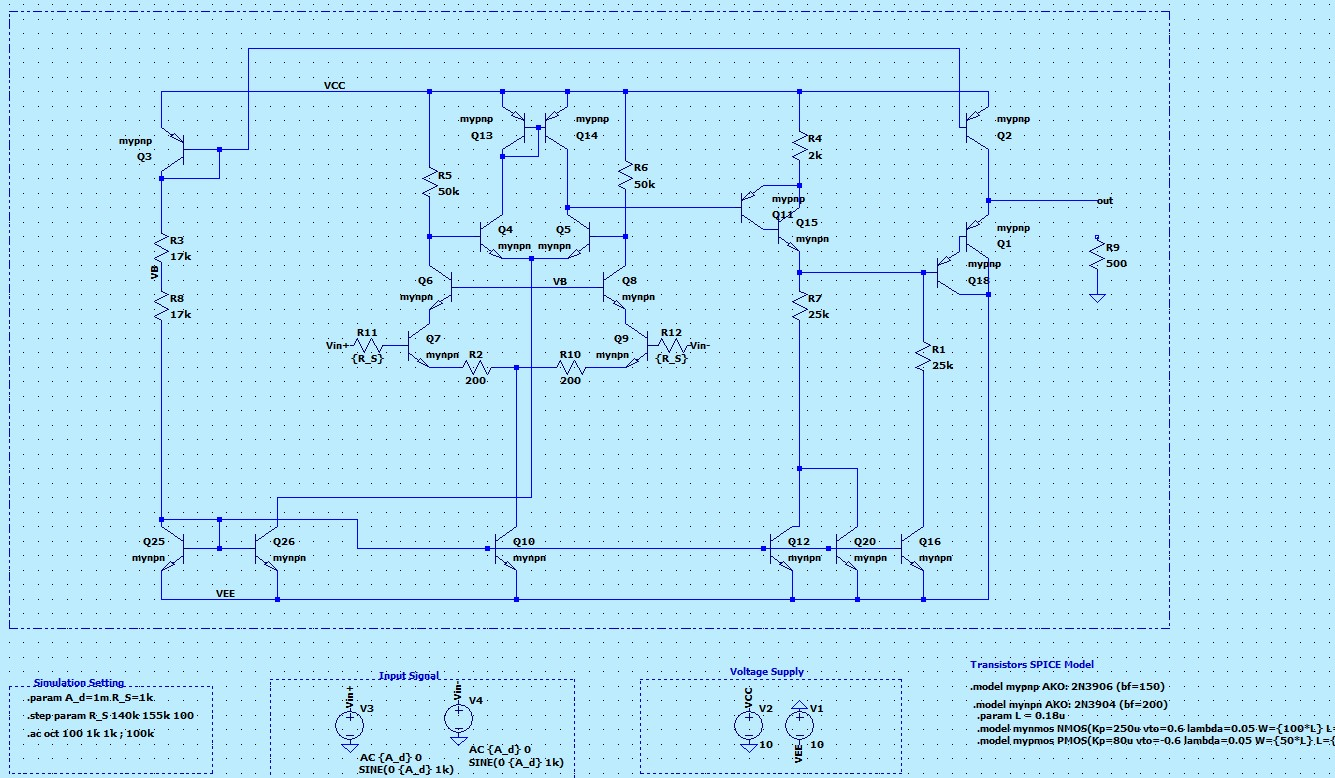
\includegraphics[width = \textwidth]{Rin_Scheme.jpg}
\end{center}
\textbf{مقدار نهایی:}
\begin{itemize}
    \item $R_{in}$: \underline{$150 \, k\Omega$}
    \item با اضافه کردن مقاومت\lr{$R_e$} در امیتر ترانزیستور‌های طبقه ورودی مقاومت ورودی چه تغییری میکند و این موضوع روی بهره‌ی تفاضلی و بهره‌ی مشترک چه تاثیری می‌گذارد؟
    مقاومت ورودی بیشتر شده و همینطور بهره مشترک را کاهش می‌دهد. با این حال تاثیر منفی بر روی بهره تفاضلی دارد.
\end{itemize}
\end{answerbox}

\newpage

% =============================================================================
% SECTION 6
% =============================================================================
\section{تحلیل مقاومت خروجی}

\begin{taskbox}{خواسته مسئله (بخش ۶)}
مقاومت خروجی مدار را بدست آورید و با شرط $R_{out}<5k\Omega$ مقایسه کنید. روش شبیه‌سازی و استخراج مقدار را توضیح دهید.
\end{taskbox}

\begin{calcbox}{محاسبات تئوری مقاومت خروجی}
مقاومت دیده شده $Q_2$ خیلی بالا بوده و در محاسبات در نظر نمی‌گیریم. هر مقاومتی که از بیس $Q_{18}$ دیده می‌شود باید تقسیم بر $\beta^2$ شود.

مقاومت دیده شده از شاخه متصل به $Q_{16}$:
$$R = 25 \text{ k}\Omega + 370  \text{ k}\Omega $$
مقاومت دیده شده از شاخه $Q_{12}$‌ $Q_{20}$ هم مقاومت یکسانی را می‌دهد. این مقاومت‌ها با مقاومت $Q_{15}$ موازی می‌شوند.
$$R_{out} = \frac{100  \text{ k}\Omega}{150^2} \approx 4  \text{ }\Omega$$
\end{calcbox}

\begin{answerbox}{نتایج شبیه‌سازی مقاومت خروجی}
ورودی را به منبع AC مناسبی متصل می‌کنیم که خروجی بدون اعوجاج به ما بدهد. یک مقاومت تست $R_L$ متصل می‌کنیم به خروجی. 
اول بدون بار ولتاژ را اندازه‌گیری می‌کنیم و اسم آن را $V_{OC}$ قرار می‌دهیم. سپس بار را وصل کرده و طوری تغییر می‌دهیم که مقدار $V_L = \frac12 V_{OC}$. آنگاه مقاومت خروجی با $R_L$ برابر است.
\begin{center}
	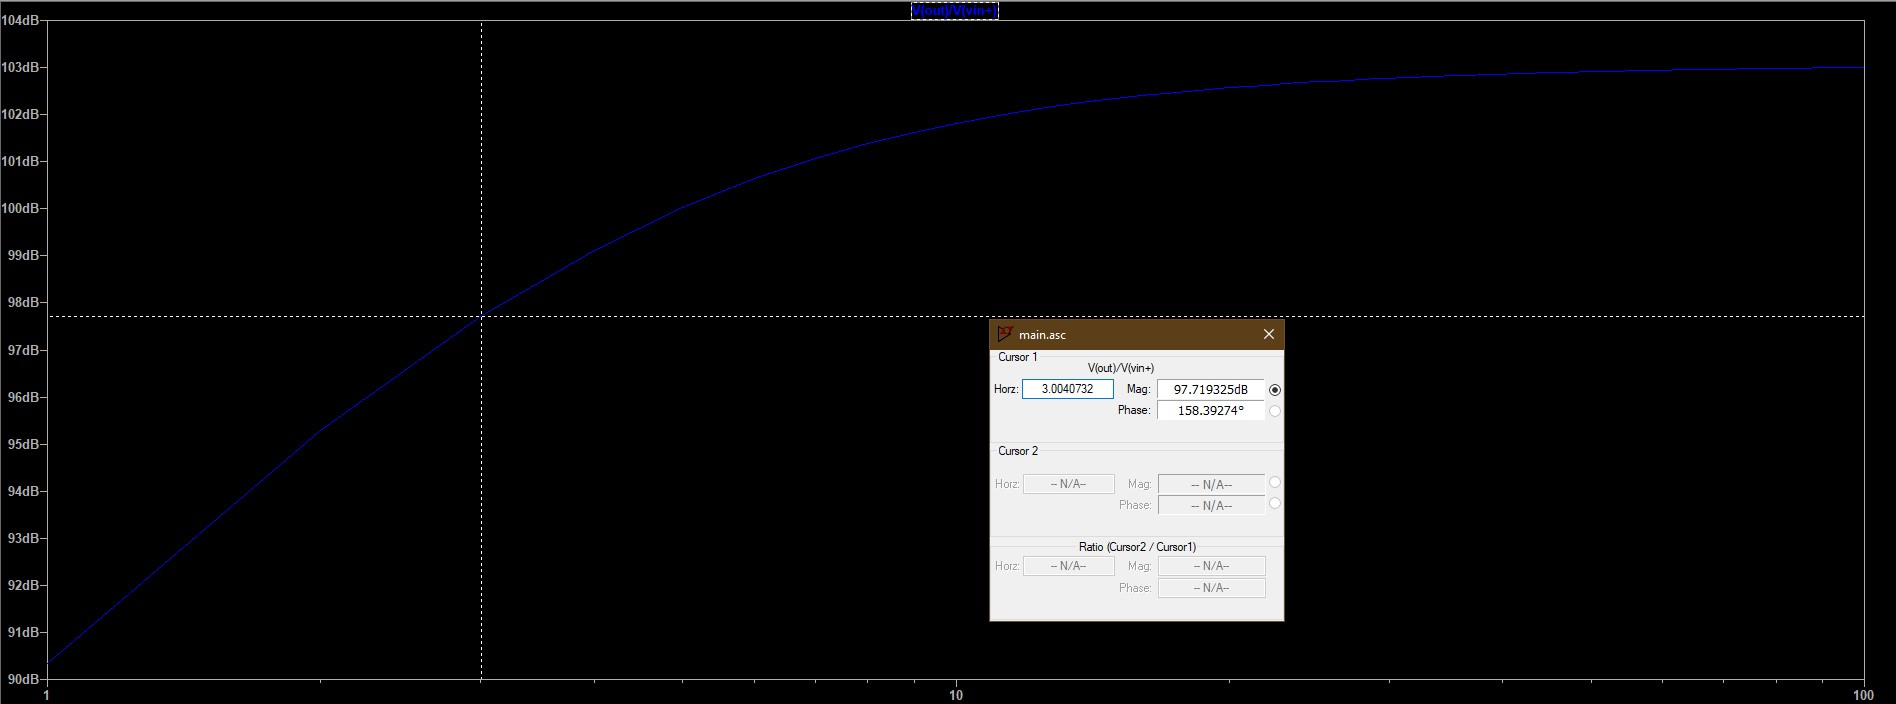
\includegraphics[width = \textwidth]{Rout_simulation.jpg}
\end{center}
\textbf{مقدار نهایی:}
\begin{itemize}
    \item $R_{out}$: \underline{$3\Omega$}
\end{itemize}
\end{answerbox}

\newpage

% =============================================================================
% SECTION 7
% =============================================================================
\section{تحلیل حوزه زمان و نوسان خروجی}

\begin{taskbox}{خواسته مسئله (بخش ۷)}
با اعمال ورودی مناسب، بررسی کنید آیا مدار می‌تواند تغییرات $6V_{pp}$ را روی بار $500\Omega$ بدون اعوجاج شدید یا کلیپینگ تأمین کند یا خیر.
\end{taskbox}

\begin{calcbox}{پیش‌بینی تئوری نوسان خروجی}
\textbf{حد بالا:}
اولین چیزی که دچار مشکل می‌شود این است با مثبت شدن مقدار ولتاژ خروجی، تمام جریان تولید شده توسط آینه جریان $Q_2$ به مقاومت رفته و باعث خاموش شدن $Q_1$ خواهد شد. 
$$V_{max} = IC_2 \times 500 \Omega = 0.3 \, V$$
\textbf{حد پایین:}
حد پایین ولتاژ زمانی می‌رسد که ولتاژ بیس $Q_{18}$ به $VEE$ می‌رسد. 
$$V_{min} = -10 + 2 \times 0.7 = -8.4 \, V$$
\vspace{5cm}
\end{calcbox}

\begin{answerbox}{نتایج شبیه‌سازی Transient}


\begin{center}

در حداکثر حالت می‌توان حدود 7 ولت سویینگ گرفت از مدار مطابق شکل زیر. 
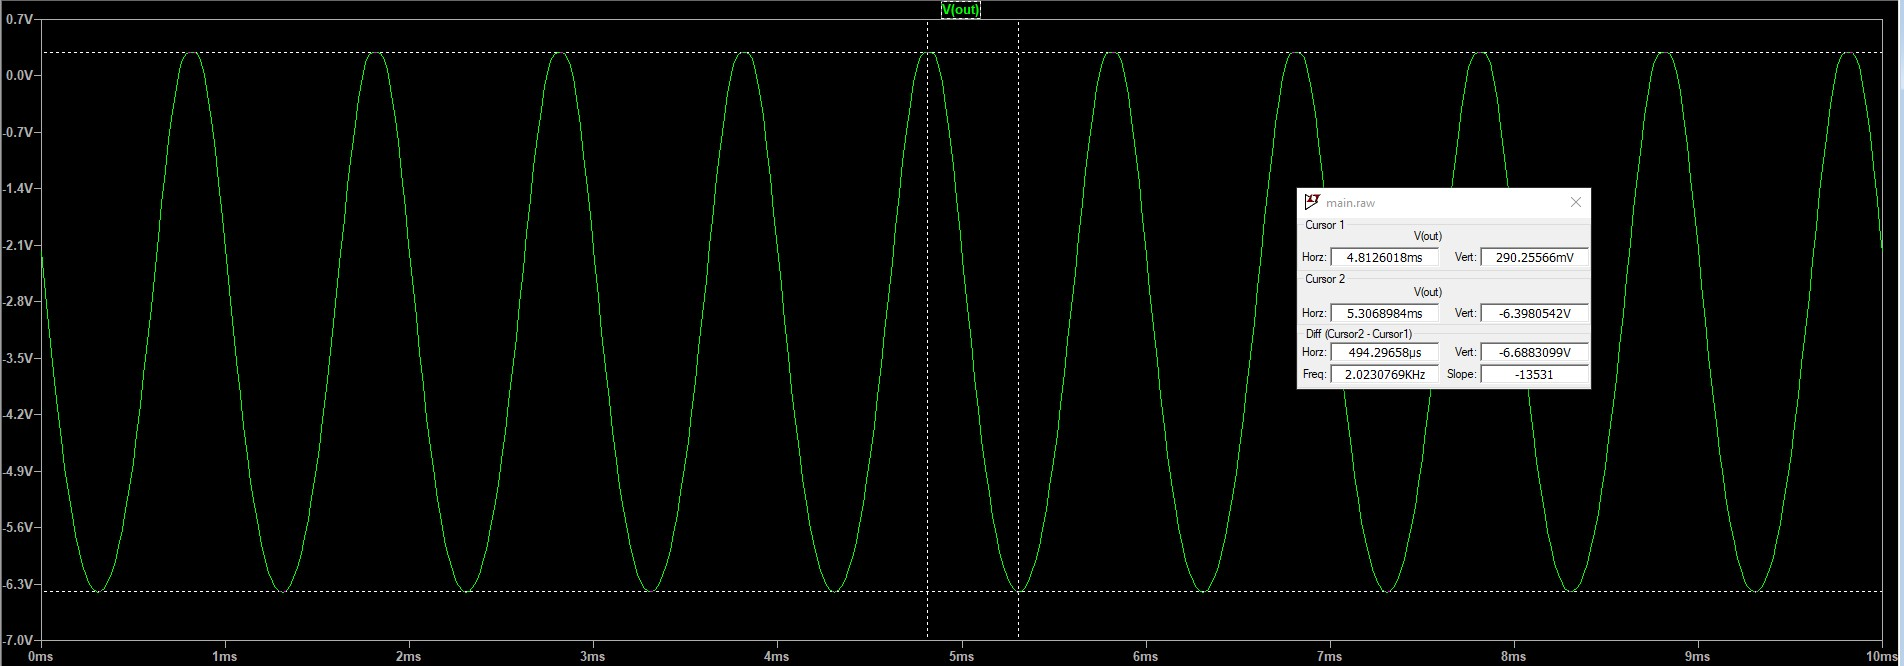
\includegraphics[width=0.85\textwidth]{Swing7v.jpg}
\end{center}

\textbf{نتیجه‌گیری:}
\begin{itemize}
    \item تغییرات خروجی پیک تا پیک: \underline{6.7}
    \item آیا در ولتاژ خروجی مناسب که شرط دامنه تغییرات خروجی را براورده میکند، خروجی دچار کلیپینگ شده است؟ \underline{خیر}
\end{itemize}
\end{answerbox}

\newpage

% =============================================================================
% SECTION 8
% =============================================================================
\section{توان مصرفی حالت سکون}

\begin{taskbox}{خواسته مسئله (بخش ۸)}
توان مصرفی حالت سکون مدار را بدون اتصال $R_{Load}$ محاسبه کنید و با شرط $P<60mW$ مقایسه نمایید.
\end{taskbox}

\begin{calcbox}{محاسبات تئوری توان}

$$P_Q = |V_{CC}I_{CC}| + |V_{EE}I_{EE}|$$
برای محاسبه‌ی توان مصرفی بدون بار، فقط کافی است جریان کشیده شده از یکی از منابع(برای مثال VCC) را اندازه گیری کنیم.
$$I_{VCC} = IC_3 + IC_6 +IC_{13} + IC_{14} + IC_{8} + IC_{15} + IC_2 = 2.48 \, \text{m}A$$
$$P = 2*I_{VCC} \times 10 = 49.6 \, mW$$
\end{calcbox}

\begin{answerbox}{نتایج شبیه‌سازی توان مصرفی}
اول بار را از روی مدار برمیداریم و سپس مقدار توان مصرفی حالت سکون را بدست می‌آوریم.

\begin{center}
\begin{tabular}{|c|c|}
\hline
\textbf{پارامتر} & \textbf{مقدار} \\
\hline
$I_{CC}$ & $2.3\, mA$\\
\hline
$I_{EE}$ &$2.4 \, mA$ \\
\hline
$P_Q$ & $47.4\, mW$\\
\hline
\end{tabular}
\end{center}

\vspace{2cm}

\end{answerbox}

\newpage

% =============================================================================
% SECTION 9
% =============================================================================
\section{محاسبه هزینه مدار}

\begin{taskbox}{خواسته مسئله (بخش ۹)}
هزینه نهایی مدار خود را با توجه به تعداد قطعات محاسبه کنید و مشخص کنید آیا بودجه $200$ واحد رعایت شده است یا خیر.
\end{taskbox}

\begin{answerbox}{جدول تعداد قطعات و هزینه}
\begin{center}
\begin{tabular}{|c|c|c|c|}
\hline
\textbf{نوع المان} & \textbf{تعداد} & \textbf{هزینه هر واحد} & \textbf{هزینه کل} \\
\hline
MOSFET &0& $3$ &0\\
\hline
BJT & 20& $5$ &100 \\
\hline
مقاومت &8 & $10$ & 80\\
\hline
خازن & 0& $40$ & 0\\
\hline
\multicolumn{3}{|c|}{\textbf{هزینه کل}} & 180\\
\hline
\end{tabular}
\end{center}

\vspace{1cm}

\textbf{آیا بودجه رعایت شده است؟} \underline{بله}

\vspace{1cm}

\textbf{در صورت استفاده از اسکریپت پایتون، خروجی آن را نیز در اینجا قرار دهید.}

\vspace{5cm}
\end{answerbox}

\newpage

% =============================================================================
% SECTION 10
% =============================================================================
\section{جمع‌بندی نهایی}

\begin{taskbox}{خواسته مسئله (بخش ۱۰)}
در یک جمع‌بندی کوتاه توضیح دهید:
\begin{itemize}
    \item مهم‌ترین چالش طراحی شما چه بود؟
    \item کدام مشخصه سخت‌تر به دست آمد؟
    \item اگر مدار شما همه مشخصات را برآورده نکرده، دلیل آن چیست؟
    \item اگر هزینه‌ی بیشتری داشتید چه بهبودی در طراحی اعمال می‌کردید؟
\end{itemize}
\end{taskbox}

\begin{answerbox}{نتیجه‌گیری نهایی}
مهم ترین چالش کنترل مقدار DC مدار و البته گین کافی جریان در خروجی بود. به دلیل آنکه از مدار \lr{Push-Pull} مجاز به استفاده نبوده‌ایم، به سختی به ساختاری دست‌یافتم که بتواند مقاومت خروجی کافی بدهد که مقدار بهره مدار نیوفتد. از طرفی مقدار DC مدار به شدت سویینگ را تحت تاثیر قرار می‌داد و در نهایت این ساختار ماکسیمم سویینگی که می‌توانیم بگیریم بدون استفاده طبقه خروجی \lr{Push-Pull} را به ما می‌دهد.
هر چند این ساختار خواسته‌های پروژه را برآورده می‌کند، ولی عملکرد فرکانسی خوبی نداره. برهره در فرکانس‌های پس از 10 کیلوهرتز سریعا کم می‌شود. 


\end{answerbox}

\end{document}
